\documentclass[pra,superscriptaddress,groupedaddress,twocolumn]{revtex4}
\usepackage{graphicx}  % needed for figures
\usepackage{siunitx}   % for decimal alignment in tables
\usepackage{bm,amssymb,amsmath}    % for math
\usepackage[bookmarks]{hyperref}
\usepackage{threeparttable}

\begin{document}

\title{Accurate predictions of ionization and atomization energies without the Born-Oppenheimer approximation}
\input{Section/authors}
\begin{abstract}
In this work we calculate the non-relativistic ground-state energies of atomic and molecular systems both with and without the Born Oppenheimer approximation. For this we utilize the fixed-node diffusion Monte Carlo method, in which the nodes depend both on the electronic and ionic positions. We report ground state energies, ionization energies and atomization energies to an accuracy of less than $1$ mHa. We find the ionization energies of the atoms to be independent of the adiabatic assumption, showing that the coupling between the nucleus and valence electrons is not important in the ionization process. The atomization energies, however, are influenced by the non-adiabatic coupling of electrons and nuclei at the sub-mHa level. We demonstrate that the fixed node approximation provides a highly accurate and scalable approach to treating molecule systems beyond the Born Oppenheimer approximation.
\end{abstract}
\maketitle

\section{Introduction}
There have been several recent discoveries~\cite{cederbaum1,gross2014,boent} that suggest that quantum wave functions, which include both electronic and ionic degrees of freedom, have many interesting properties that have yet to be explored.  This includes the development of equations that exactly factorize a wave function into electron and ionic components~\cite{cederbaum1}, the disappearance of conical intersections in wave functions of model systems~\cite{gross2014}, and the use of quantum entanglement to study electronic and ionic density matrices~\cite{boent}.  Extending such studies to realistic systems is of broad interest and will considerably expand our understanding of electron-ion systems. However, treatment of \textit{ab initio} electron-ion systems is challenging and applications have thus been limited.   The most accurate simulations of electron-ion wave functions are generally done with very specialized wave functions, which are limited to rather small systems \cite{mitroy2013}.  

As a framework to address these problems in general realistic systems, we recently demonstrated that quantum Monte Carlo (QMC) can be combined with quantum chemistry techniques to generate electron-ion wave functions~\cite{Tubman_ECG}.  We treated realistic molecular systems and demonstrated that our method can be scaled to larger systems than previously considered while maintaining a highly accurate wave function. In the following we extend our previous work by considering the simulation of a larger benchmark set of atoms and molecules.  We calculate ionization energies and dissociation energies which can be directly compared with previous benchmarking results.  We also consider using multiple time steps for different species in the imaginary time propagator, which is also developed and tested.  %Additionally we consider other estimators and the errors associated by using a mixed estimator.

\section{Method}
\subsection{Fixed-Node Diffusion Monte Carlo (FN-DMC)}
Diffusion Monte Carlo is a projector method that evolves a trial wavefunction in imaginary time and projects out the ground-state wavefunction.  For practical simulations of fermions, the fixed-node approximation is introduced, which depends only on set of electronic positions where a trial wave functions is equal to zero.  This approximation is different than approximations typically used in quantum chemistry calculations, and in this work we demonstrate that we can generate high quality nodal surfaces for a range of systems which include full electron-ion wave functions. 

In the limiting case that the trial wavefunction has the same nodal surface as the exact ground-state wavefunction, FN-DMC can be applied to obtain the exact ground-state energy.  Approximate nodal surface can be generated through optimization of the full wave function. Such approximate nodal surfaces have been tested and validated on a wide range of systems, and consistently provide an excellent approximation of the exact ground-state energy,  comparable to the state of the art in \textit{ab initio} simulations~\cite{grossman1}. In addition the energies generated with FN-DMC are variational with regards to the ground state energy.

%With advances in wave function optimization, 
In all but a handful of previous QMC simulations, ions are "clamped" to their equilibrium positions. Recent advances~\cite{Nightingale_Linear,Umrigar_Linear,Brown_Bench} have made it possible to optimize thousands of wave function parameters simultaneously with variational Monte Carlo within the clamped nuclei approximation. However, Such an assumption is not fundamentally required by FN-DMC.  In our previous work we found that the most important effect to optimize for were the nodes due to electron-electron correlations~\cite{Tubman_ECG}, and in this regard we use more sophisticated electronic terms in the wave function than the ion part of the wave function.

\subsection{Electron Wavefunction and Optimization}
There are several different approaches for generating high quality wave functions ~\cite{Umrigar_Alleviation,Toulouse_Bench, Brown_Bench,Seth_Bench}. We use an initial guess for the wavefunction that is generated from complete active space self-consistent field (CASSCF) \cite{Chaban_MCSCF,Szabo} calculation using the quantum chemistry package GAMESS \cite{GAMESS}. The optimized orbitals are then used in a second order configuration interaction (SOCI) calculation to generate a series of configuration state functions (CSF)~\cite{Clark_Bench}. The multi-CSF expansion of the wavefunction  can be expressed in the following form,
\begin{align}
\Psi_{SOCI}(\vec{r})=\sum\limits_{i=1}^{N_{CSF}}\alpha_i\phi_i(\vec{r}), \label{eq:psi_gms}
\end{align}
where $\vec{r}$ refers to the spacial coordinates of all the electrons. $\phi_i(\vec{r})$ are the CSF generated from SOCI. We used the cc-pV5Z basis for all the atomic systems and Roos Augmented Triple Zeta ANO basis for molecular systems~\cite{dunning,roos}. We then impose cusp condition on each molecular orbital~\cite{cusp} and add a Jastrow factor to the wave function to include electron correlation~\cite{Kato}. Our Jastrow factor contains one, two and three body terms. The full wave function being optimized is then
\begin{align}
\Psi_e(\vec{r})=e^{J(\vec{r},\vec{\beta})}\sum\limits_{i=1}^{N_{CSF}}\alpha_i\phi_i(\vec{r})\label{eq:psie}
\end{align}
We optimized the CSF and Jastrow coefficients $\vec{\alpha},\vec{\beta}$ simultaneously with QMCPACK \cite{QMCPACK}.

\subsection{Electron-Ion Wavefunction}

\begin{figure}[t]
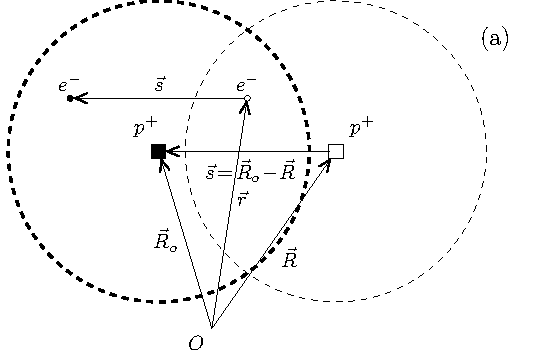
\includegraphics[width=9cm]{fig1a.pdf}
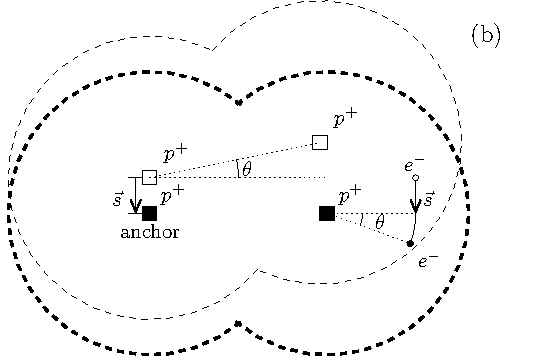
\includegraphics[width=9cm]{fig1b.pdf}
\caption{ Symmetries for simulation of atomic and molecule systems in QMC {\bf (a)} For atomic systems we can consider the entire wavefunction shifting with the ion. This process can be visualized by following a contour of the wavefunction. The thick dashed circle represents a contour of the electron wavefunction when the proton is at its reference position $\vec{R}_o$ and the thin dashed circle represents the same contour when the proton has moved to a new position $\vec{R}$. To evaluate the ion-dependent electron wavefunction $\bar{\psi}_e(\vec{r},\vec{R})$, we simply map the electron to its proper place in the reference wavefunction $\psi_e(\vec{r})$. That is, $\bar{\psi}_e(\vec{r},\vec{R})=\bar{\psi}_e(\vec{r}+\vec{s},\vec{R}_o)=\psi_e(\vec{r}+\vec{s})$ where $\vec{s}$ is the shift required to put the proton back to its reference position. {\bf (b)} For H$_2^+$, we pick one of the protons as an "anchor" and approximate the new wavefunction by dragging the reference wavefunction with the "anchor" proton. We also rotate the wavefunction to align its axis of symmetry with the orientation of the two protons. \label{fig:drag}}
\end{figure}

Once a satisfactory electronic wave function has been obtained, we construct the electron-ion wave function using the ansatz we previously investigated~\cite{Tubman_ECG},
\begin{align}
\Psi_{ei}(\vec{r},\vec{R})=\psi_I(\vec{R})\bar{\psi}_e(\vec{r},\vec{R}), \label{eq:psi}
\end{align}
where $\vec{R}$ includes spatial coordinates of all ions. The ion wave function consists of simple products of Gaussian wave functions over each nuclei pair,
\begin{align}
\psi_I(\vec{R})\propto \prod\limits_{i,i<j}e^{-a(\vert \vec{R}-\vec{R}_j\vert-b_{ij})^2},
\label{wfs_ions}
\end{align}
where $a$ is a contraction coefficient for the ion wave function that we optimize for each system and $b_{ij}$ are taken to be the equilibrium distances between the nuclei at the minimum of the potential energy surface of the clamped nuclei.  Due to the locality of the Gaussian basis set used in the quantum chemistry calculations for constructing the electronic wave function, the nodes change based on the ionic position, which we have previously called the dragged-node approximation.  Although there are approaches for going beyond this approximation, it was demonstrated to be highly accurate over a range of molecules in previous work.  For the systems considered here, we can impose various symmetries of the Hamiltonian onto the wave function that arise from the relative motion of the ions.  In Fig.~\ref{fig:drag} we demonstrate this strategy for the simple cases of a hydrogen atom and a H$_2^+$ molecular ion. Although the dragged-node technique is developed with atomic and diatomic systems in mind, it is not difficult to generalize it for use in larger systems or even apply to parts of a bigger system, e.g., treating light ions as quantum particles and heavy ions as "clamped".

\section{Results and Discussion}
\begin{table*}[t!]
\setlength{\extrarowheight}{1pt}
\begin{threeparttable}
\caption{Ground state energies for atoms and ions, and the ionization energies: Fixed-Node DMC results of this work (FN-DMC) for atoms and ions with and without the adiabatic assumption. The ionization potentials (IP) are reported in the last section of the table with the experimental values. Energies are given in units of Hartree. \label{tab:ionization}}
\begin{tabular*}{\textwidth}{@{\extracolsep{\fill}} c*{10}{D{.}{.}{6}} }
\hline\hline
Atom & .$Li$(^2$S$) & .$Be$(^1$S$) & .$B$(^2$P$) & .$C$(^3$P$) & .$N$(^4$S$) & .$O$(^3$P$) & .$F$(^2$P$) \\ \hline
&&.$clamped$&$nuclei$&&&& \\
FN-DMC & -7.478056(4) & -14.66732(1) & -24.65377(1) & -37.84449(2) & -54.58858(3) & -75.06576(4) & -99.7316(1) \\
Seth DMC \cite{Seth_Bench} & -7.478067(5) & -14.667306(7) & -24.65379(3) & -37.84446(6) & -54.58867(8) & -75.0654(1) & -99.7318(1) \\
Davidson 1993 \cite{Davidson_Atoms} &  -7.47807 & -14.66736 & -24.65391 & -37.8450 &-54.5892 & -75.0673 & -99.7339 \\
&&&non.$adiabatic$&&&& \\
FN-DMC & -7.47742(1) & -14.66643(2) & -24.65244(3) & -37.84277(6) & -54.58655(8) & -75.0631(1) & -99.7290(4) \\
\hline
Ion & .$Li$^+(^1$S$) & .$Be$^+(^2$S$) & .$B$^+(^1$S$) & .$C$^+(^2$P$) & .$N$^+(^3$P$) & .$O$^+(^4$S$) & .$F$^+(^3$P$) \\ \hline
&&.$clamped$&$nuclei$&&&& \\
FN-DMC & -7.279919(4) & -14.324753(6) & -24.34884(1) & -37.43075(2) & -54.05376(3) & -74.56588(4) & -99.0913(1) \\
Seth DMC \cite{Seth_Bench} & -7.279914(3) & -14.324761(3) & -24.34887(2) & -37.43073(4) & -54.05383(7) & -74.56662(7) & -99.0911(2) \\
Davidson 1993 \tnote{a} \cite{Davidson_Atoms} & -7.27999 & -14.3249 & -24.3489 & -37.4312 & -54.0552 & -74.5668 & -99.0937 \\
&&&non.$adiabatic$&&&& \\
FN-DMC & -7.2793(1) & -14.32386(2) & -24.34750(3) & -37.42904(4) & -54.05182(9) & -74.56336(8) & -99.0885(3) \\
\hline
&&.$clamped$&$nuclei$&&&& \\
IP (FN-DMC) & 0.19814(1) & 0.34257(1) & 0.30493(1) & 0.41374(3) & 0.53482(4) & 0.49988(5) & 0.6403(1) \\
&&&non.$adiabatic$&&&& \\
IP (FN-DMC) & 0.1981(1) & 0.34257(3) & 0.30494(4) & 0.41373(7) & 0.5347(1) & 0.4997(1) & 0.6405(5) \\
IP (Exp.) \cite{CCCBDB} & 0.19808 & 0.3425 & 0.30502 & 0.413797 & 0.533967 & 0.500526 & 0.640173 \\
\hline\hline
\end{tabular*}
\begin{tablenotes}
\item[a] The ionic ground state energies are calculated by adding ionization potentials in Table XII to the atomic ground state energies in Table XI from Ref.~\cite{Davidson_Atoms}.
\end{tablenotes}
\end{threeparttable}
\end{table*}

\begin{figure}
\centering
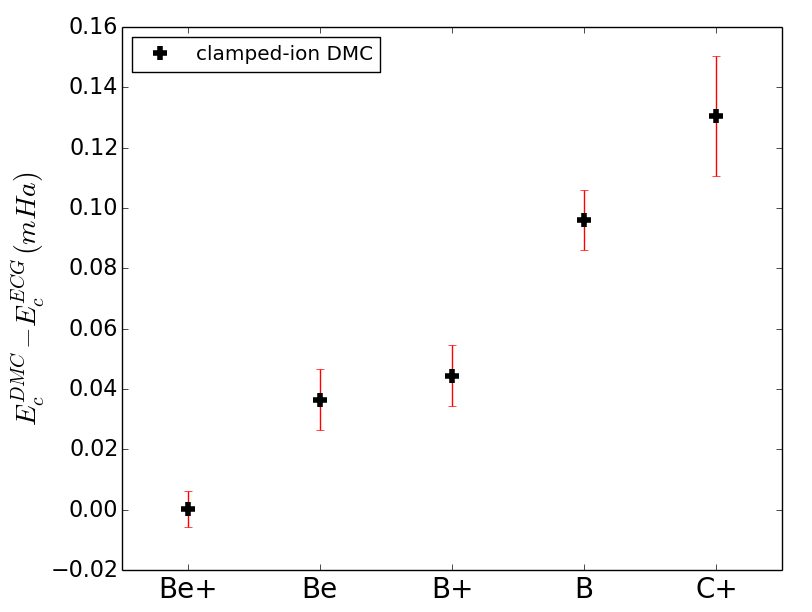
\includegraphics[scale=.4]{Figures/ad-ECG}
\caption{Ground state energy of Be,$\text{Be}^+$,B,$\text{B}^+$ and $\text{C}^+$ calculated with clamped-ion FN-DMC compared to ECG results.~\cite{Stanke_Be,Puchalski_Be+,Bubin_B,Bubin_B+,Bubin_C+} The ECG reference energies are chosen to be the origins of the y-axes. \label{fig:ad-atoms}}
\end{figure}

\begin{figure}
\centering
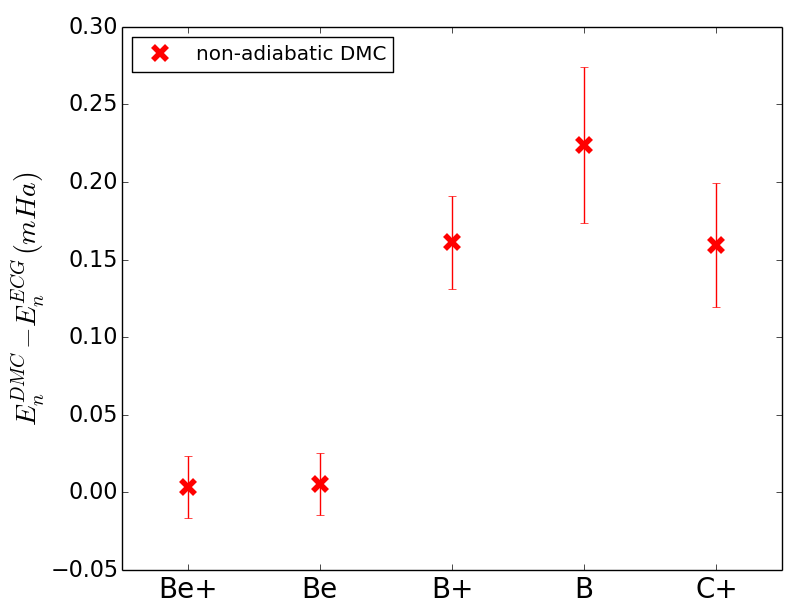
\includegraphics[scale=.4]{Figures/nad-ECG}
\caption{Ground state energy of Be,$\text{Be}^+$,B,$\text{B}^+$ and $\text{C}^+$ calculated with non-adiabatic FN-DMC compared to ECG results.~\cite{Bubin_BeH_noBO,Bubin_B,Bubin_B+,Bubin_C+} The ECG reference energies are chosen to be the origins of the y-axes. \label{fig:nad-atoms}}
\end{figure}

\subsection{Ground State Energies}
Ground state energies are calculated for first row atoms and ions and hydrides with and without the adiabatic assumption, see Table \ref{tab:ionization} and \ref{tab:atomization}. The ground state geometries for BeH and BH are chosen to be the ECG-optimized distances for a comparison with the ECG method and the geometries for the rest of the hydrides are taken from experimental data \cite{CCCBDB}. For the systems, Li, Be, B, Be$^+$, B$^+$, C$^+$ and LiH the ECG/Hylleraas results are converged to several digits beyond what can be done with normal quantum chemistry techniques.  Thus these results are likely much more accurate than experimental results, and are converged to an accuracy beyond our FN-DMC results.   %For the largest ECG simulation of the BH molecule, it is clear that this high level of convergence has not been achieved, as our QMC results are significantly lower in energy.  
   We first perform a CAS(m,n) calculation (m electrons into n active orbitals), then the MCSCF optimized orbitals are used in a SOCI calculation that includes single and double excitations of the m electrons into all of the remaining valance orbitals. We include all CSFs with coefficients bigger than some cutoff $\epsilon$ to lend reasonable flexibility to the wavefunction during optimization. We include as many CSFs as possible to maximize the flexibility of the wavefunction. However, the inclusion of too many CSFs with small expansion coefficients can introduces noise as they requires a large number of samples in the optimization step to be optimized. We have chosen $\epsilon$ to restrict the number of CSFs in the wave function to be $\sim$1000 in all systems. Optimization was performed with the linear method with roughly $10^7$ statistically independent samples and we chose a cost function consisting of equal parts average local energy and reweighted variance. We performed timestep extrapolation for all of the tested systems. At least four timesteps from $0.005~\text{Ha}^{-1}$ to $0.001~\text{Ha}^{-1}$ were used for all systems in the adiabatic FN-DMC.

As an illustration of the high quality QMC techniques used in this work, we compare our atomic results with a recent QMC benchmark study~\cite{Seth_Bench}. The clamped nuclei ground state FN-DMC energies are consistently equal across all systems (except for O$^{+}$), within error bars. This is an interesting coincidence since we used a different approach in optimizing our wave functions. In particular our large multi-determinant expansions, can be compared with the approach used by Seth {\it et al.}~\cite{Seth_Bench} which used moderately-sized multi-determinant expansions ($\sim$ 100 CSF) with a backflow transformation.   
 
For the atomic systems, there are three ECG calculations of non-adiabatic ground state energies we can use as benchmark. The non-adiabatic ground-state energies for Be, $\text{Be}^+$, B,$\text{B}^+$ and $\text{C}^+$ are in agreement with ECG results (-14.66643544~Ha~\cite{Bubin_BeH_noBO},-14.32386349~Ha~\cite{Bubin_BeH_noBO},-24.65262387(250)~Ha~\cite{Bubin_B},-24.347641289(35)~Ha~\cite{Bubin_B+},-37.42916955(250)~Ha~\cite{Bubin_C+}) within 0.2 mHa as shown in Figure \ref{fig:ECG-atoms} .

We performed a study over diatomic systems, the results of which are presented in Table \ref{tab:atomization}. For these diatomic systems, there are high quality thermochemistry benchmark results for which we can compare ~\cite{Feller_Corrections}. 

To make the comparison against the thermochemistry benchmark results, we take the reference energies from the last column of Table VI of Ref.~\cite{Feller_Corrections} and subtracted the corrections in the $\Delta E_{SR}$ and SO columns for comparison with our non-adiabatic energies.  For the comparison with our adiabatic energies we subtracted the DBOC and ZPE corrections.  Corrections from spin-orbit coupling and relativistic effects are not used, as they are not included in our Hamiltonian.

\subsection{Ionization Energies}

\begin{figure}[h]
\centering
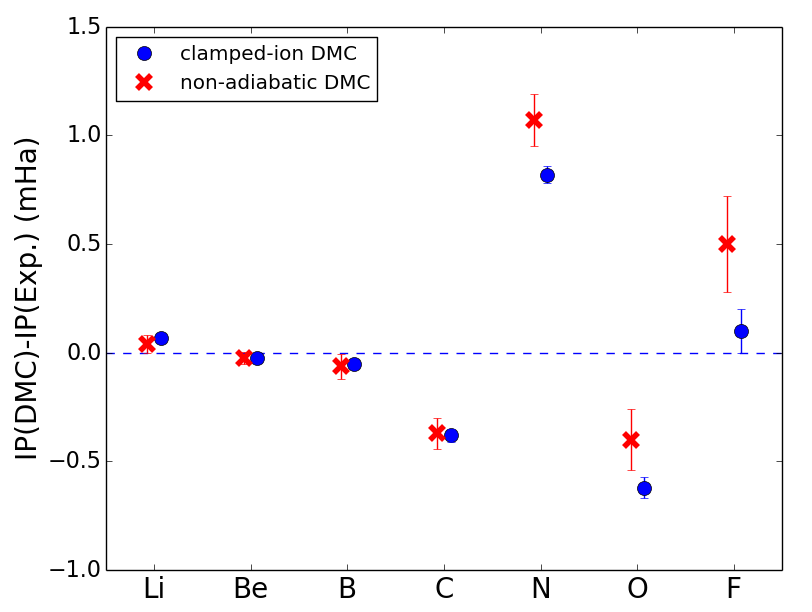
\includegraphics[scale=.4]{Figures/ionization}
\caption{Calculated ionization energies compared to experimental data. The calculated energies are all within 1 mHa of experiment.}
\end{figure}

The ionization energies are listed in Table \ref{tab:ionization}.  Notice that even though ground state energies change significantly with the inclusion of non-adiabatic effects, the ionization energies match with or without the adiabatic assumption. This suggests that for atomic systems, coupling between valence electron and ion motions is small. The difference in ground state energies can be entirely attributed to the zero point motion of the nuclei. Physically, this means that for all first row atoms, the outer most electron is screened from the nucleus and all of the energy required for its removal can be attributed to its interaction with the rest of the electrons in the atom.

For the LiH molecule we are also interested in calculating the electron affinity for comparison to ECG results. We calculated the ground state energy of LiH$^-$ to be $-8.08220(2)$~Ha for the case of clamped nuclei.  With non-adiabatic effects included our result is  $-8.07811(3)$~Ha. Our non-adiabatic result is in good agreement with a previous ECG study \cite{Bubin_LiH_noBO} which reported a value of $-8.07856887$~Ha. We report an electron affinity of $0.01191(4)$~Ha which is can be compared to the ECG prediction of $0.012132(2)$~Ha and agrees with experiment, $0.0126(4)$~Ha. \footnote{We note that LiH ground state energies which we compare against are mislabeled in Ref.\cite{Bubin_LiH_noBO}, with $\text{LiH}^-$ and LiD being switched.}

\subsection{Atomization Energies}

\begin{figure}
\centering
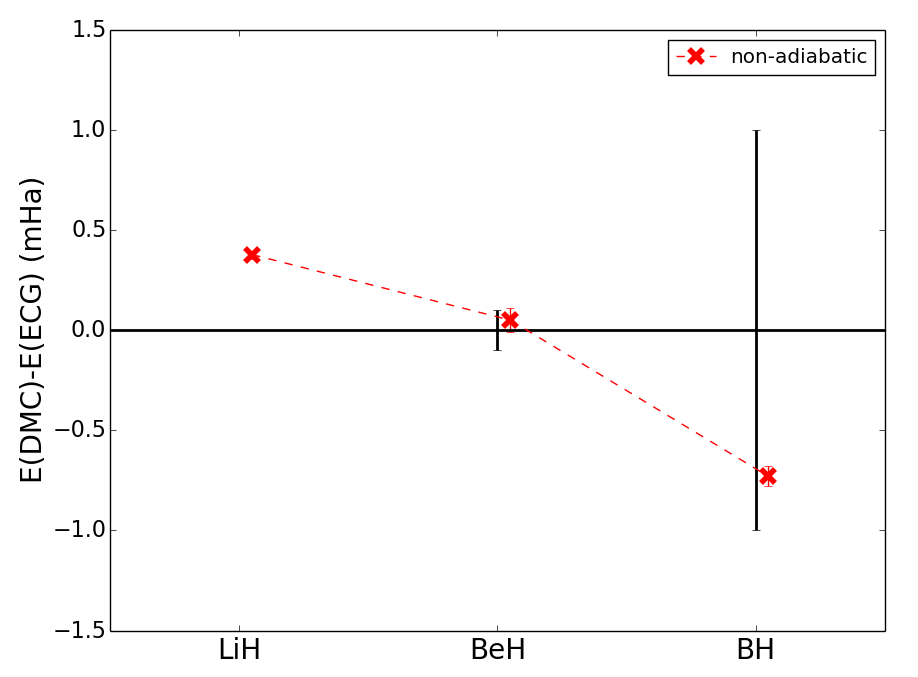
\includegraphics[scale=.4]{Figures/dia-ECG}
\caption{Ground state energy of LiH, BeH and BH calculated with non-adiabatic FN-DMC compared to ECG results.~\cite{Adamowicz_LiH,Koput_BeH,Miliordos_BH} The ECG reference energies are chosen to be the origins of the y-axes.}
\end{figure}

\begin{figure}
\centering
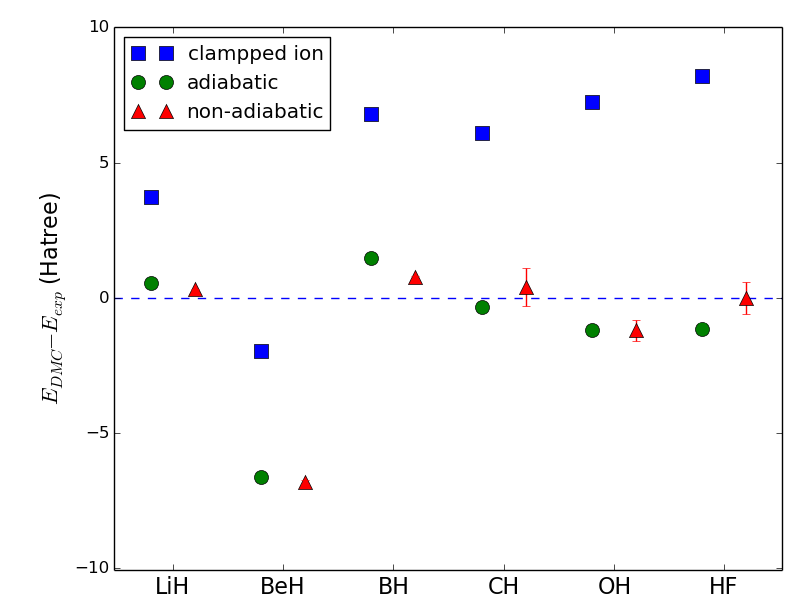
\includegraphics[scale=.4]{Figures/atomization}
\caption{Atomization energies of first row hydrides obtained with FN-DMC. The adiabatic results are estimated by adding zero-point energies from \cite{Feller_Corrections} to the clamped nuclei energies as exact corrections. Experimental values are chosen to be the origins of the y-axis.}
\end{figure}

The ground state energies for various hydrides are reported in Table \ref{tab:atomization}. The energies calculated for clamped nuclei are on par with the best available quantum chemistry results \cite{Adamowicz_LiH,Koput_BeH,Miliordos_BH}. The energies calculated without the adiabatic assumption are in agreement with the ECG results for LiH, BeH to within 0.4 mHa. For small systems, ECG results are typically orders of magnitude more accurate than the best QMC and quantum chemistry simulations. However, with BH being one of the largest ECG simulations performed, the QMC results are actually lower in energy, in this case by 1 mHa. For the systems CH, OH, and HF, there are no explicit simulations we can compare against, and we rely on the experimental results and the results with estimated non-adiabatic corrections for comparison. Our biggest errors appear to occur for BeH and OH.   For the case of BeH our agree with accuracy higher than 1 mHa with both the ECG results and semi-empirical benchmarking. In particular the ECG results are converged to more digits than the experimental error bar, and it is likely the experimental reference has errors on the order of 5 mHa.   For the case of OH, our error is on the order of 1 mHa, which isn't unexpected as our clamped nuclei ground state energy is roughly 3 mHa from the actual estimated ground state energy.
 
\begin{table*}[t!]
\setlength{\extrarowheight}{1pt}
\begin{threeparttable}
\caption{Ground-state energies and atomization energies: fixed-node DMC results of this work for all first row hydrides with and without the Born-Oppenheimer approximation. The rows marked with bolded \textbf{FN-DMC} are our non-adiabatic results. All atomization energies are all estimated for 0K. $D_o$ includes zero-point energy contribution while $D_e$ does not. Energies are given in units of Hartree. \label{tab:atomization}}
\begin{tabular}
% siunitx setup
{
 l
 S[table-format=1.6]
 S[table-format=4.6]
 S[table-format=4.6]
 S[table-format=4.6]
 S[table-format=4.6]
 S[table-format=4.6]
 S[table-format=4.6]
}

\hline\hline
\multicolumn{1}{c}{Molecule} & 
\multicolumn{1}{c}{LiH$(^1\Sigma^+)$} &
\multicolumn{1}{c}{BeH$(^2\Sigma^+)$} &
\multicolumn{1}{c}{BH$(^1\Sigma^+)$} &
\multicolumn{1}{c}{CH$(^2\Pi)$} &
\multicolumn{1}{c}{OH$(^2\Pi)$} &
\multicolumn{1}{c}{HF$(^1\Sigma^+)$} \\ 
\hline
\multicolumn{1}{c}{} & 
\multicolumn{1}{c}{} &
\multicolumn{1}{c}{} &
\multicolumn{1}{c}{clamped-nuclei} &
\multicolumn{1}{c}{} &
\multicolumn{1}{c}{} &
\multicolumn{1}{c}{} \\
FN-DMC & \text{-}8.070518(2) & \text{-}15.24793(2) & \text{-}25.28867(2) & \text{-}38.47801(4) & \text{-}75.7357(1) & \text{-}100.4552(1) \\
$E_{\text{ref}}$ \tnote{a} & \text{-}8.0705473 & \text{-}15.2483(4) & \text{-}25.2893(2) & \text{-}38.4792(2) & \text{-}75.7382(2) & \text{-}100.4600(3) \\
\multicolumn{1}{c}{} & 
\multicolumn{1}{c}{} &
\multicolumn{1}{c}{} &
\multicolumn{1}{c}{non-adiabatic} &
\multicolumn{1}{c}{} &
\multicolumn{1}{c}{} &
\multicolumn{1}{c}{} \\
\textbf{FN-DMC} & \text{-}8.06624(2) & \text{-}15.24194(4) & \text{-}25.28102(2) & \text{-}38.46721(3) & \text{-}75.72453(9) & \text{-}100.44315(7) \\
ECG \cite{Bubin_LiH_noBO,Bubin_BeH_noBO,Bubin_BH_noBO} & \text{-}8.0664371(15) & \text{-}15.24203(10) & \text{-}25.2803(10) & N/A & N/A & N/A \\
\hline

\multicolumn{1}{c}{} & 
\multicolumn{1}{c}{} &
\multicolumn{1}{c}{} &
\multicolumn{1}{c}{clamped-nuclei} &
\multicolumn{1}{c}{} &
\multicolumn{1}{c}{} &
\multicolumn{1}{c}{} \\
$D_e$ (this work) & 0.09246(1) & 0.08062(2) & 0.13493(3) & 0.13353(5) & 0.1699(1) & 0.2234(1) \\
$D_e$ Feller \tnote{b} & 0.09262(5) & 0.0809(4) & 0.1354(2) & 0.1342(2) & 0.1709(2) & 0.2258(3) \\
\multicolumn{1}{c}{} & 
\multicolumn{1}{c}{} &
\multicolumn{1}{c}{} &
\multicolumn{1}{c}{non-adiabatic} &
\multicolumn{1}{c}{} &
\multicolumn{1}{c}{} &
\multicolumn{1}{c}{} \\
$D_o$ (this work) & 0.08908(4)  & 0.07578(4)  & 0.12890(4) & 0.12480(9) & 0.1617(1) & 0.2141(1) \\
$D_o$ Feller \tnote{c} & 0.08940(5) & 0.0761(4) & 0.1299(2) & 0.1276(2) & 0.1622(2) & 0.2166(3)\\
$D_o$ Exp. \cite{CCCBDB,HH} & 0.08874(38) & 0.07475(4) & 0.1281(37)\tnote{d} & 0.1275(5) & 0.1622(1) & 0.2158(3) \\
\hline\hline
\end{tabular}
\begin{tablenotes}
\item[a] For LiH, ECG provides the best reference energy~\cite{Adamowicz_LiH}. For the rest of the systems, we combined the best clamped-ion atomic references in Table \ref{tab:ionization} and thermochemistry estimates of $D_e$ in this table to produce the reference ground-state energies.
\item[b] Best estimates for $D_e$ are calculated by subtracting the scalar relativistic, spin-orbit coupling and zero-point energy corrections from the reference $D_o$ in Table VI of Ref.~\cite{Feller_Corrections}.
\item[c] Here only the scalar relativistic and spin-orbit coupling corrections are subtracted.
\item[d] The atomization energy for BeH in Ref.~\cite{CCCBDB} disagrees with previous high level theoretical benchmarks~\cite{Feller_Corrections,Bubin_BeH_noBO}, thus we use Ref.~\cite{HH} instead.
\end{tablenotes}
\end{threeparttable}
\end{table*}

\section{Conclusion}
We calculated the ground-state energies of first row atoms and their corresponding ions and hydrides to an accuracy of $0.1$ mHa both with and without the adiabatic assumption. We found the ionization energies of the atoms to be independent of the adiabatic assumption, suggesting that the energy difference between the adiabatic and non-adiabatic ground states is due to the zero point motion of the nuclei at the energy scales of interest. The atomization energies of simple hydrides, however, were significantly different in the adiabatic than in the non-adiabatic limit.   We showed that it is necessary to include non-adiabatic effects to accurately predict the experimental values of atomization energies for these simple hydrides.

These calculations also verified the validity of our wave function ansatz, namely it does indeed produce a high quality electron-ion trial wavefunction from a good electron wavefunction. This technique also has the potential to solve interesting larger-scale problems due to its ease of implementation as well as the polynomial scaling in computational time with respect to the number of electrons.  This technique can be generalized quite easily to deal with larger systems.

\section{Acknowledgment}
The authors would like to thank Mike Pak, Kurt Brorsen, Katharina Doblhoff-Dier and Brian Busemeyer for useful discussions. The authors would also like to thank Prof. Willem Klopper for providing the DBOC references for the atoms and ions and Prof. David Feller for providing the DBOC data for the hydrides. This work was supported by the U.S. Department of Energy grant No. 1-485267-244000-191100 as part of the Scientific Discovery through Advanced Computing (SciDAC) program. We used the Extreme Science and Engineering Discovery Environment (XSEDE), which is supported by the National Science Foundation Grant No. OCI-1053575 and resources of the Oak Ridge Leadership Computing Facility (OLCF) at the Oak Ridge National Laboratory, which is supported by the Office of Science of the U.S. Department of Energy under Contract No. DE-AC05-00OR22725.

\bibliography{ref}
\end{document}
